%!TEX program = xelatex


\documentclass[onecolumn,a4paper,10pt]{article}

\usepackage[ boldfont,slantfont]{xeCJK}  %设定支持中文
\usepackage{multicol}

\graphicspath{{figures/}}    %设置放置图片的文件夹

\linespread{1.2}     %设置行间距的命令

\setmainfont{Times New Roman}

%for windows fonts
%\setCJKmainfont[BoldFont={SimHei},ItalicFont={KaiTi}]{SimSun}
%\setsansfont{SimHei}
%
%\setCJKfamilyfont{song}{SimSun}
%\setCJKfamilyfont{kai}{KaiTi}
%\setCJKfamilyfont{hei}{SimHei}
%\setCJKfamilyfont{yao}{FZYaoTi}
%
%\newcommand\song{\CJKfamily{song}}
%\newcommand\kai{\CJKfamily{kai}}
%\newcommand\hei{\CJKfamily{hei}}
%\newcommand\yao{\CJKfamily{yao}}

\setCJKmainfont[BoldFont={STXihei},ItalicFont={STKaiti}]{STSong}
\setsansfont{STXihei}

\setCJKfamilyfont{song}{STSong}
\setCJKfamilyfont{kai}{STKaiti}
\setCJKfamilyfont{hei}{STXihei}
%\setCJKfamilyfont{yao}{FZYaoTi}

\newcommand\song{\CJKfamily{song}}
\newcommand\kai{\CJKfamily{kai}}
\newcommand\hei{\CJKfamily{hei}}
%\newcommand\yao{\CJKfamily{yao}}

\newcommand{\erhao}{\fontsize{22pt}{\baselineskip}\selectfont}
\newcommand{\xiaoerhao}{\fontsize{18pt}{\baselineskip}\selectfont}
\newcommand{\sanhao}{\fontsize{16pt}{\baselineskip}\selectfont}
\newcommand{\xiaosanhao}{\fontsize{15pt}{\baselineskip}\selectfont}
\newcommand{\sihao}{\fontsize{14pt}{\baselineskip}\selectfont}
\newcommand{\xiaosihao}{\fontsize{12pt}{\baselineskip}\selectfont}
\newcommand{\wuhao}{\fontsize{10.5pt}{\baselineskip}\selectfont}
\newcommand{\xiaowuhao}{\fontsize{9pt}{\baselineskip}\selectfont}
\newcommand{\liuhao}{\fontsize{7.5pt}{\baselineskip}\selectfont}

%%%段落首行缩进两个字
\makeatletter
\let\@afterindentfalse\@afterindenttrue
\@afterindenttrue
\makeatother
\setlength{\parindent}{2em}%中文缩进两个汉字位

\newcommand{\tabincell}[2]{\begin{tabular}{@{}#1@{}}#2\end{tabular}}

%%%%%%%%%% 定理类环境的定义 %%%%%%%%%%
%% 必须在导入中文环境之后
\newtheorem{example}{例}             % 整体编号
\newtheorem{algorithm}{算法}
\newtheorem{theorem}{定理}[section]  % 按 section 编号
\newtheorem{definition}{定义}
\newtheorem{axiom}{公理}
\newtheorem{property}{性质}
\newtheorem{proposition}{命题}
\newtheorem{lemma}{引理}
\newtheorem{corollary}{推论}
\newtheorem{remark}{注解}
\newtheorem{condition}{条件}
\newtheorem{conclusion}{结论}
\newtheorem{assumption}{假设}

%%%%%%%%%% 一些重定义 %%%%%%%%%%
%% 必须在导入中文环境之后
\renewcommand{\contentsname}{目录}     % 将Contents改为目录
\renewcommand{\abstractname}{摘\ \ 要} % 将Abstract改为摘要
\renewcommand{\refname}{参考文献}      % 将References改为参考文献
\renewcommand{\indexname}{索引}
\renewcommand{\figurename}{图}
\renewcommand{\tablename}{表}
\renewcommand{\appendixname}{附录}
%\renewcommand{\proofname}{证明}
\renewcommand{\algorithm}{算法}

%%%%%%%%%%%%%%%%%%%%%%%%%%%%%%%%%%%%%%%%%%%%%%%%%%%%%%%%%%%%%%%%
%  packages
%    这部分声明需要用到的包
%%%%%%%%%%%%%%%%%%%%%%%%%%%%%%%%%%%%%%%%%%%%%%%%%%%%%%%%%%%%%%%%
\usepackage{graphicx}    % EPS 图片支持
\usepackage{indentfirst} % 中文段落首行缩进
\usepackage{bm}          % 公式中的粗体字符(用命令\boldsymbol)
\usepackage{graphics}	%让文档支持图片
\usepackage{amsmath}	%ams可以让文档支持数学公式
\usepackage{fancyhdr}
\usepackage{fontspec,xunicode,xltxtra}
\usepackage{hyperref}	%让文档支持超链接
\usepackage{booktabs}	%让文档支持三线表格
\usepackage{amsfonts}
\usepackage{amssymb}
\usepackage{color}
\usepackage{graphicx,psfrag}
\usepackage{epsfig}
\usepackage{verbatim}
\usepackage{picins}
\usepackage{multirow}
\usepackage{listings}
\usepackage{xcolor}
\usepackage[titletoc]{appendix} %附件支持


%%%%%%%%%%%%%%%%%%%%%%%%%%%%%%%%%%%%%%%%%%%%%%%%%%%%%%%%%%%%%%%%
%  lengths
%    下面的命令重定义页面边距,使其符合中文刊物习惯。
%%%%%%%%%%%%%%%%%%%%%%%%%%%%%%%%%%%%%%%%%%%%%%%%%%%%%%%%%%%%%%%%
\addtolength{\topmargin}{-54pt}
\setlength{\oddsidemargin}{0.63cm}  % 3.17cm - 1 inch
\setlength{\evensidemargin}{\oddsidemargin}
\setlength{\textwidth}{14.66cm}
\setlength{\textheight}{24.00cm}    % 24.62
\begin{document}
%%%%%%%%%%%%%%%%%%%%%%%%%%%%%%%%%%%%%%%%%%%%%%%%%%%%%%%%%%%%%%%%
%  定义标题格式,包括title,author,affiliation,email等。
%  在任何用到中文的地方,用\begin{CJK} ... \end{CJK}将其括起来。
%%%%%%%%%%%%%%%%%%%%%%%%%%%%%%%%%%%%%%%%%%%%%%%%%%%%%%%%%%%%%%%%
\title{\hei{磁锁定效果测试 }}
\author{肖波\footnote{xbustc@gmail.com}~~~~~~
\\[8pt]
\xiaowuhao 合肥微尺度物质科学国家实验室,安徽~~合肥~~230026\\[4pt]
}
%\date{\today}  % 这一行用来去掉默认的日期显示
\date{\today}
%%%%%%%%%%%%%%%%%%%%%%%%%%%%%%%%%%%%%%%%%%%%%%%%%%%%%%%%%%%%%%%%
%  自定义命令
%%%%%%%%%%%%%%%%%%%%%%%%%%%%%%%%%%%%%%%%%%%%%%%%%%%%%%%%%%%%%%%%
% 此行使文献引用以上标形式显示
\newcommand{\supercite}[1]{\textsuperscript{\cite{#1}}}
%%%%%%%%%%%%%%%%%%%%%%%%%%%%%%%%%%%%%%%%%%%%%%%%%%%%%%%%%%%%%%%%
%  显示title,并设页码为空(按杂志社要求)
%%%%%%%%%%%%%%%%%%%%%%%%%%%%%%%%%%%%%%%%%%%%%%%%%%%%%%%%%%%%%%%%
\maketitle
\pagestyle{fancy}
\lhead{磁场锁定}
\cfoot{\thepage}
\thispagestyle{empty}
%\pagestyle{empty} \thispagestyle{empty}
\vspace{-20pt}

%%%%%%%%%%%%%%%%%%%%%%%%%%%%%%%%%%%%%%%%%%%%%%%%%%%%%%%%%%%%%%%%
%  中文摘要
%%%%%%%%%%%%%%%%%%%%%%%%%%%%%%%%%%%%%%%%%%%%%%%%%%%%%%%%%%%%%%%%

\begin{center}
\parbox{\textwidth}{
%\rule{2em}{0pt}
\hei{摘要:}\song{在超冷原子相关的实验中,磁场的稳定性会极大的影响原子的退相干时间,因此,在大部分的超冷原子实验中都会配备PID反馈系统用以稳定原子的偏置磁场,延长相干时间。本方案基于海德堡光晶格实验室目前采用的方案,用以稳定原子的任意方向偏置磁场。}\\[5pt]
\hei{关键词:}\song{磁锁定;PID;反馈控制}
\\[5pt]
}
\end{center}

\tableofcontents

\newpage



\iffalse
%%%%%%%%%%%%%%%%%%%%%%%%%%%%%%%%%%%%%%%%%%%%%%%%%%%%%%%%%%%%%%%%
%  英文摘要
%%%%%%%%%%%%%%%%%%%%%%%%%%%%%%%%%%%%%%%%%%%%%%%%%%%%%%%%%%%%%%%%
\begin{center}
\sihao{\textbf{A \LaTeX{} Template for Chinese Reports}}\\[7pt]
\normalsize
Weiyong Zhang~~~~~~
\\[7pt]
\xiaowuhao Hefei National Laboratory for Physical Sciences at the Microscale, HeFei, AnHui, 230026\\[10pt]
\end{center}
\begin{center}
\parbox{\textwidth}{
\textbf{Abstract:} This is a \LaTeX{} template used for writting documents in Chinese form.\\[4pt]
\textbf{Keywords:} Key; Key; the Key
}
\end{center}
\fi

\section{实验规划}
在超晶格中,我们往往需要将某些格点上的原子通过$\pi/2$的微波脉冲将原子在0和1态之间翻转,磁场的噪声会影响两个态之间的能量差,从而影响态制备的fidelity。而我们的磁场锁定系统将用于在提供偏置磁场的同时抑制这个磁场噪声,从而提高相应的态制备的fidelity。

我们最后science腔是有Kimball Physics提供的八边形金属腔,金属的涡流和磁性将会为磁场锁定将会带来一定的问题。spin-dependent的晶格对偏置磁场的方向有一定依耐性,所以为了让晶格在dependent和非dependent之间转换,有时需要将偏置磁场旋转90度,所以我们计划在三个方向都加上sensor选择性补偿单一方向,多方向同时补可能会导致竞争降低补偿效果,摆放位置如图\ref{place}。

\begin{figure}[htbp]
\centering
\includegraphics[width=3in]{sensorplace}
\caption{fluxgate固定图}
\label{place}
\end{figure}

我们的补偿线圈结构如图\ref{frame}。我们将在每一个方向都绕两对亥姆霍兹线圈,一对匝数为2的动态补偿线圈和一对匝数为20的偏置线圈。各个方向上1A电流对应的理论产生磁场值如表格\ref{magnetic}。

\begin{figure}[htbp]
\centering
\includegraphics[width=3in]{磁补偿frame}
\caption{反馈补偿线圈框架示意图}
\label{frame}
\end{figure}

\begin{table}[htbp]
\centering

\label{magnetic}
\begin{tabular}{|c|c|c|c|}
\hline
方向&长宽& 距离&  1A对应磁场大小\\
\hline
竖直& 26*26 cm &  21.3 cm&\tabincell{c}{20匝: 901 mG \\2匝: 90.1 mG}\\
\hline
水平X & 22*23 cm & 12 cm&\tabincell{c}{20匝: 1485 mG \\2匝: 148.5 mG}\\
\hline
水平Y & 24*23 cm & 12 cm&\tabincell{c}{20匝: 1437 mG \\2匝: 143.7 mG}\\
\hline
\end{tabular}
\caption{线圈参数}
\end{table}

我们将会采用双极性电流源N175提供偏置磁场,足以使磁场大小达到1G左右。

\section{实验材料}

\subsection{双极性电流源}

为了产生偏置磁场,需要在补偿线圈中加入电流。电流的稳定性一定程度上决定了偏置磁场锁定的最终效果。我们已经从Highfinesse订购了两台BCS5/10,输出最大为5A/10V,电流噪声小于$2.5*10^{-5}*Imax$,同时它可以接受±10V内的模拟信号调整输出电流大小,这个功能对于反馈控制非常重要.但是目前这两台还未到货,测试时我们使用的是海德堡workshop做的自制双极性电流源N175,测试得出的RMS噪声大小在$1.5*10^{-4} A$左右,输出电流最大为2A,最大控制电压为5V。

\subsection{Fluxgate}
实验中我们使用StefanMayer公司生产的FL1-200型号Fluxgate测量环境中的磁场大小以获得PID反馈中的误差信号。其磁场测量范围为±2Gauss,频响范围为1kHz,输出为±10V对应±2Gauss,基本可以满足我们未来实验的需求。

\subsection{Coils}
我们的线圈由一对10匝的偏置线圈和一对2匝的补偿线圈构成。其中匝数较低的补偿线圈由于电感较小,频率响应较好,相位延迟低,所以用以动态补偿磁场漂移。对于偏置线圈,加一定电流产生一定的偏置磁场,它工作时产生的磁场噪声与环境噪声一起被动态补偿线圈通过PID反馈控制进行抑制。线圈大小约为26*26cm,距离也为20cm左右,为了模拟最后竖直方向上的补偿效果。经过测量,对补偿线圈通以1A电流,相应的能产生92.5mG的磁场,对于偏置线圈,这个值是500mG。

\subsection{Adwin时序控制系统}
实验中我们使用的是软件PID,将测量值和设定值取差,在CPU中根据预设定好的P,I,D大小,利用离散PID算法\begin{equation}
u(i)=Kp*e(i)+Ki*\sum_{k=0}^{i}e(k)+Kd*[e(k)-e(k-1)]
\end{equation}
设定输出给双极性电源源控制电压的大小。这一功能由时序控制系统Adwin来完成,它的CPU主频为300Mhz,最小处理时间间隔为3ns,同时它有一个18位的模拟输入模块和多块16位模拟输出模块。整个软件PID的反馈控制逻辑如图\ref{fig1:PID}。

\begin{figure}[htbp]
\centering
\includegraphics[width=6in]{PIDMAG}
\caption{反馈控制逻辑}
\label{fig1:PID}
\end{figure}

%\subsection{Agilent数字万用表}
%我们采用Agilent的数字万用表34410精度为六位半,最小采样间隔为0.05ms。由于它精度高,我们用它来测试fluxgate的输出,以观测磁场的变化。

\section{实验过程}
\subsection{N175测试结果}
\subsubsection{Agilent数字万用表和Adwin模拟输入端口并联测量}
我们用数字万用表测试了在偏置线圈加电流和不加电流时环境磁场的大小,RMS噪声大小没有太大的区别,同时在频谱上看二者也基本没有太大区别,说明偏置线圈产生的磁场噪声较小,且没有太大的白噪声,也没有特别大的高频噪声,可以通过动态补偿进行消除。在测试时我们一般不使用偏置线圈,只使用动态补偿线圈。

经过简单的一些测试比较,在ADwin执行的算法中我们设定Adwin每隔10us采集一次fluxgate的测量数据,同时为了减小ADwin自身的测量误差,我们设定采集20次求的平均值作为测量值与设定值相减得到误差信号再通过离散PID算法计算得到输出信号。所以ADwin每隔200us输出一次控制信号去锁定磁场,这个速度已经足够覆盖由于fluxgate频宽范围和线圈的响应频宽决定的最后有效锁定频宽。

我们测试了未锁定前的环境磁场大小作为对比的标准,设定P,I,  D的值为3,1.2,0.5后,发现RMS噪声从未锁定前的0.76mG抑制到0.22mG,数据点和频谱图如图\ref{fig:1022}.

\begin{figure}[htbp]
\centering
\includegraphics[height=1.5in]{DataMultimeter}%
\hspace{0.4in}%   (表示两张图片的中间间距,其中的%不可缺失)
\includegraphics[height=1.75in]{FourierMultimeter}
\caption{锁定前后磁场数据与频谱对比图}
\label{fig:1022}
\end{figure}

其中数据点的纵轴单位为电压,表示fluxgate的输出电压,与磁场的转换关系为200mG/V。从数据点图上可以看到,锁定后磁场的变化范围从0.02V缩小到0.003V,PID反馈的效果基本达到我们的预期。从频谱图上看,环境噪声除了由于市电导致的50Hz以及50Hz倍频的特定噪声成分,在14.2Hz左右也有比较高的噪声功率,这说明在我们的实验室附近有一个以14.2Hz运转的电气设备,但这个来源目前尚未找到。同时,可以看到在300Hz以下,锁定对这些特定噪声成分都有明显的抑制,但是比较无法理解的是即使在低频范围内白噪声都没有被抑制,反而得到了加强。

我们首先怀疑PID反馈控制的算法导致了这个问题的产生,我们尝试更换PID的值,以及改变ADWIN数据采集速度和输出控制信号速度等方法,虽然频谱线会发生改变,但是白噪声始终未得到抑制。

最后我们改进了我们的ADwin执行算法,将ADwin采集的20次平均出的测量值输出,得出ADwin的数据采集结果如图\ref{fig:1029}(P,I,D=2.4,3.3,2.75).
\begin{figure}[htbp]
\centering
\includegraphics[height=1.5in]{DataAdwin}%
\hspace{0.4in}%   (表示两张图片的中间间距,其中的%不可缺失)
\includegraphics[height=1.75in]{FourierAdwin}
\caption{锁定前后ADWIN磁场数据与频谱对比图}
\label{fig:1029}
\end{figure}

这里再次列出同时刻万用表测出数据的频谱图\ref{fig:Multimeter2}.

\begin{figure}[htbp]
\centering
\includegraphics[height=2in]{Multimeter2}
\caption{Agilent数字万用表结果}
\label{fig:Multimeter2}
\end{figure}


ADwin结果显示RMS噪声由1.02mG抑制到0.18mG。从数据点图上看变化范围和之前用数字万用表测试的结果基本一致,对于频谱图来说,ADwin的结果显示,在300Hz以下,无论是白噪声和特定频率噪声成分都得到了很好的抑制。但同时,Agilent数字万用表的结果与ADwin结果无论是在锁定前还是锁定后的频谱都存在很大差异。

可能存在的原因:

\begin{itemize}
\item 由于并联,ADwin的输入端口在万用表输入端口引入了一定噪声。
\item ADwin的测量端口被PID反馈回路所影响,得到的数据让ADwin认为自身已经达到最好的补偿效果,这个时候ADwin达到了稳定工作的状态。
\end{itemize}

\subsubsection{双fluxgate隔离测量}
为了确定到底是ADwin的问题还是万用表的问题,我们在以下测量中,数字万用表和Adwin的输入端口隔离,这种情况下无法让数字万用表和Adwin同时测量同一个fluxgate,所以我们在锁定时使用的fluxgate旁边距离1cm左右的地方放入第二个fluxgate,用数字万用表采集这个fluxgate的输出电压,同时通过测量这个fluxgate,我们也可以验证虽然锁定时测量的是单点的磁场,但是有效锁定的范围并不局限于这个点。

最后数字万用表和ADwin的测试结果如下:
\begin{figure}[htbp]
\centering
\includegraphics[height=1.5in]{Data-Sep-multimeter}%
\hspace{0.4in}%   (表示两张图片的中间间距,其中的%不可缺失)
\includegraphics[height=1.75in]{Fourier-Sep-multimeter}
\caption{锁定前后数字万用表磁场数据与频谱对比图}
\label{fig:1105}
\end{figure}

图\ref{fig:1105} RMS噪声:1.26mG->0.28mG

\begin{figure}[htbp]
\centering
\includegraphics[height=1.5in]{Data-Sep-Adwin}%
\hspace{0.4in}%   (表示两张图片的中间间距,其中的%不可缺失)
\includegraphics[height=1.75in]{Fourier-Sep-Adwin}
\caption{锁定前后ADWIN磁场数据与频谱对比图}
\label{fig:1104}
\end{figure}

图\ref{fig:1104} RMS噪声:1.28mG->0.32mG

从上面的图,我们可以看到的是,结果和之前并联时几乎没有差别。这也就说明两者端口的并联并不是万用表和ADwin的频谱结果有如此大的差异的原因。

为了进一步验证PID反馈回路是否有影响,我们用ADwin另一个不参与PID反馈控制的输入端口取代万用表测试第二个fluxgate的输出端口,结果图\ref{fig:1203}。
\newpage
\begin{figure}[htbp]
\centering
\includegraphics[height=1.5in]{Data-Sensor2-Adwin}%
\hspace{0.4in}%   (表示两张图片的中间间距,其中的%不可缺失)
\includegraphics[height=1.75in]{Fourier-Sensor2-Adwin}
\caption{锁定前后ADWIN通道2磁场数据与频谱对比图}
\label{fig:1203}
\end{figure}
图\ref{fig:1203} RMS噪声:1.38mG->0.42mG

作为比较,同时刻,通道1测量的锁定用的fluxgate磁场数据如图\ref{fig:1204}。

\begin{figure}[htbp]
\centering
\includegraphics[height=1.5in]{Data-Sensor1-Adwin}%
\hspace{0.4in}%   (表示两张图片的中间间距,其中的%不可缺失)
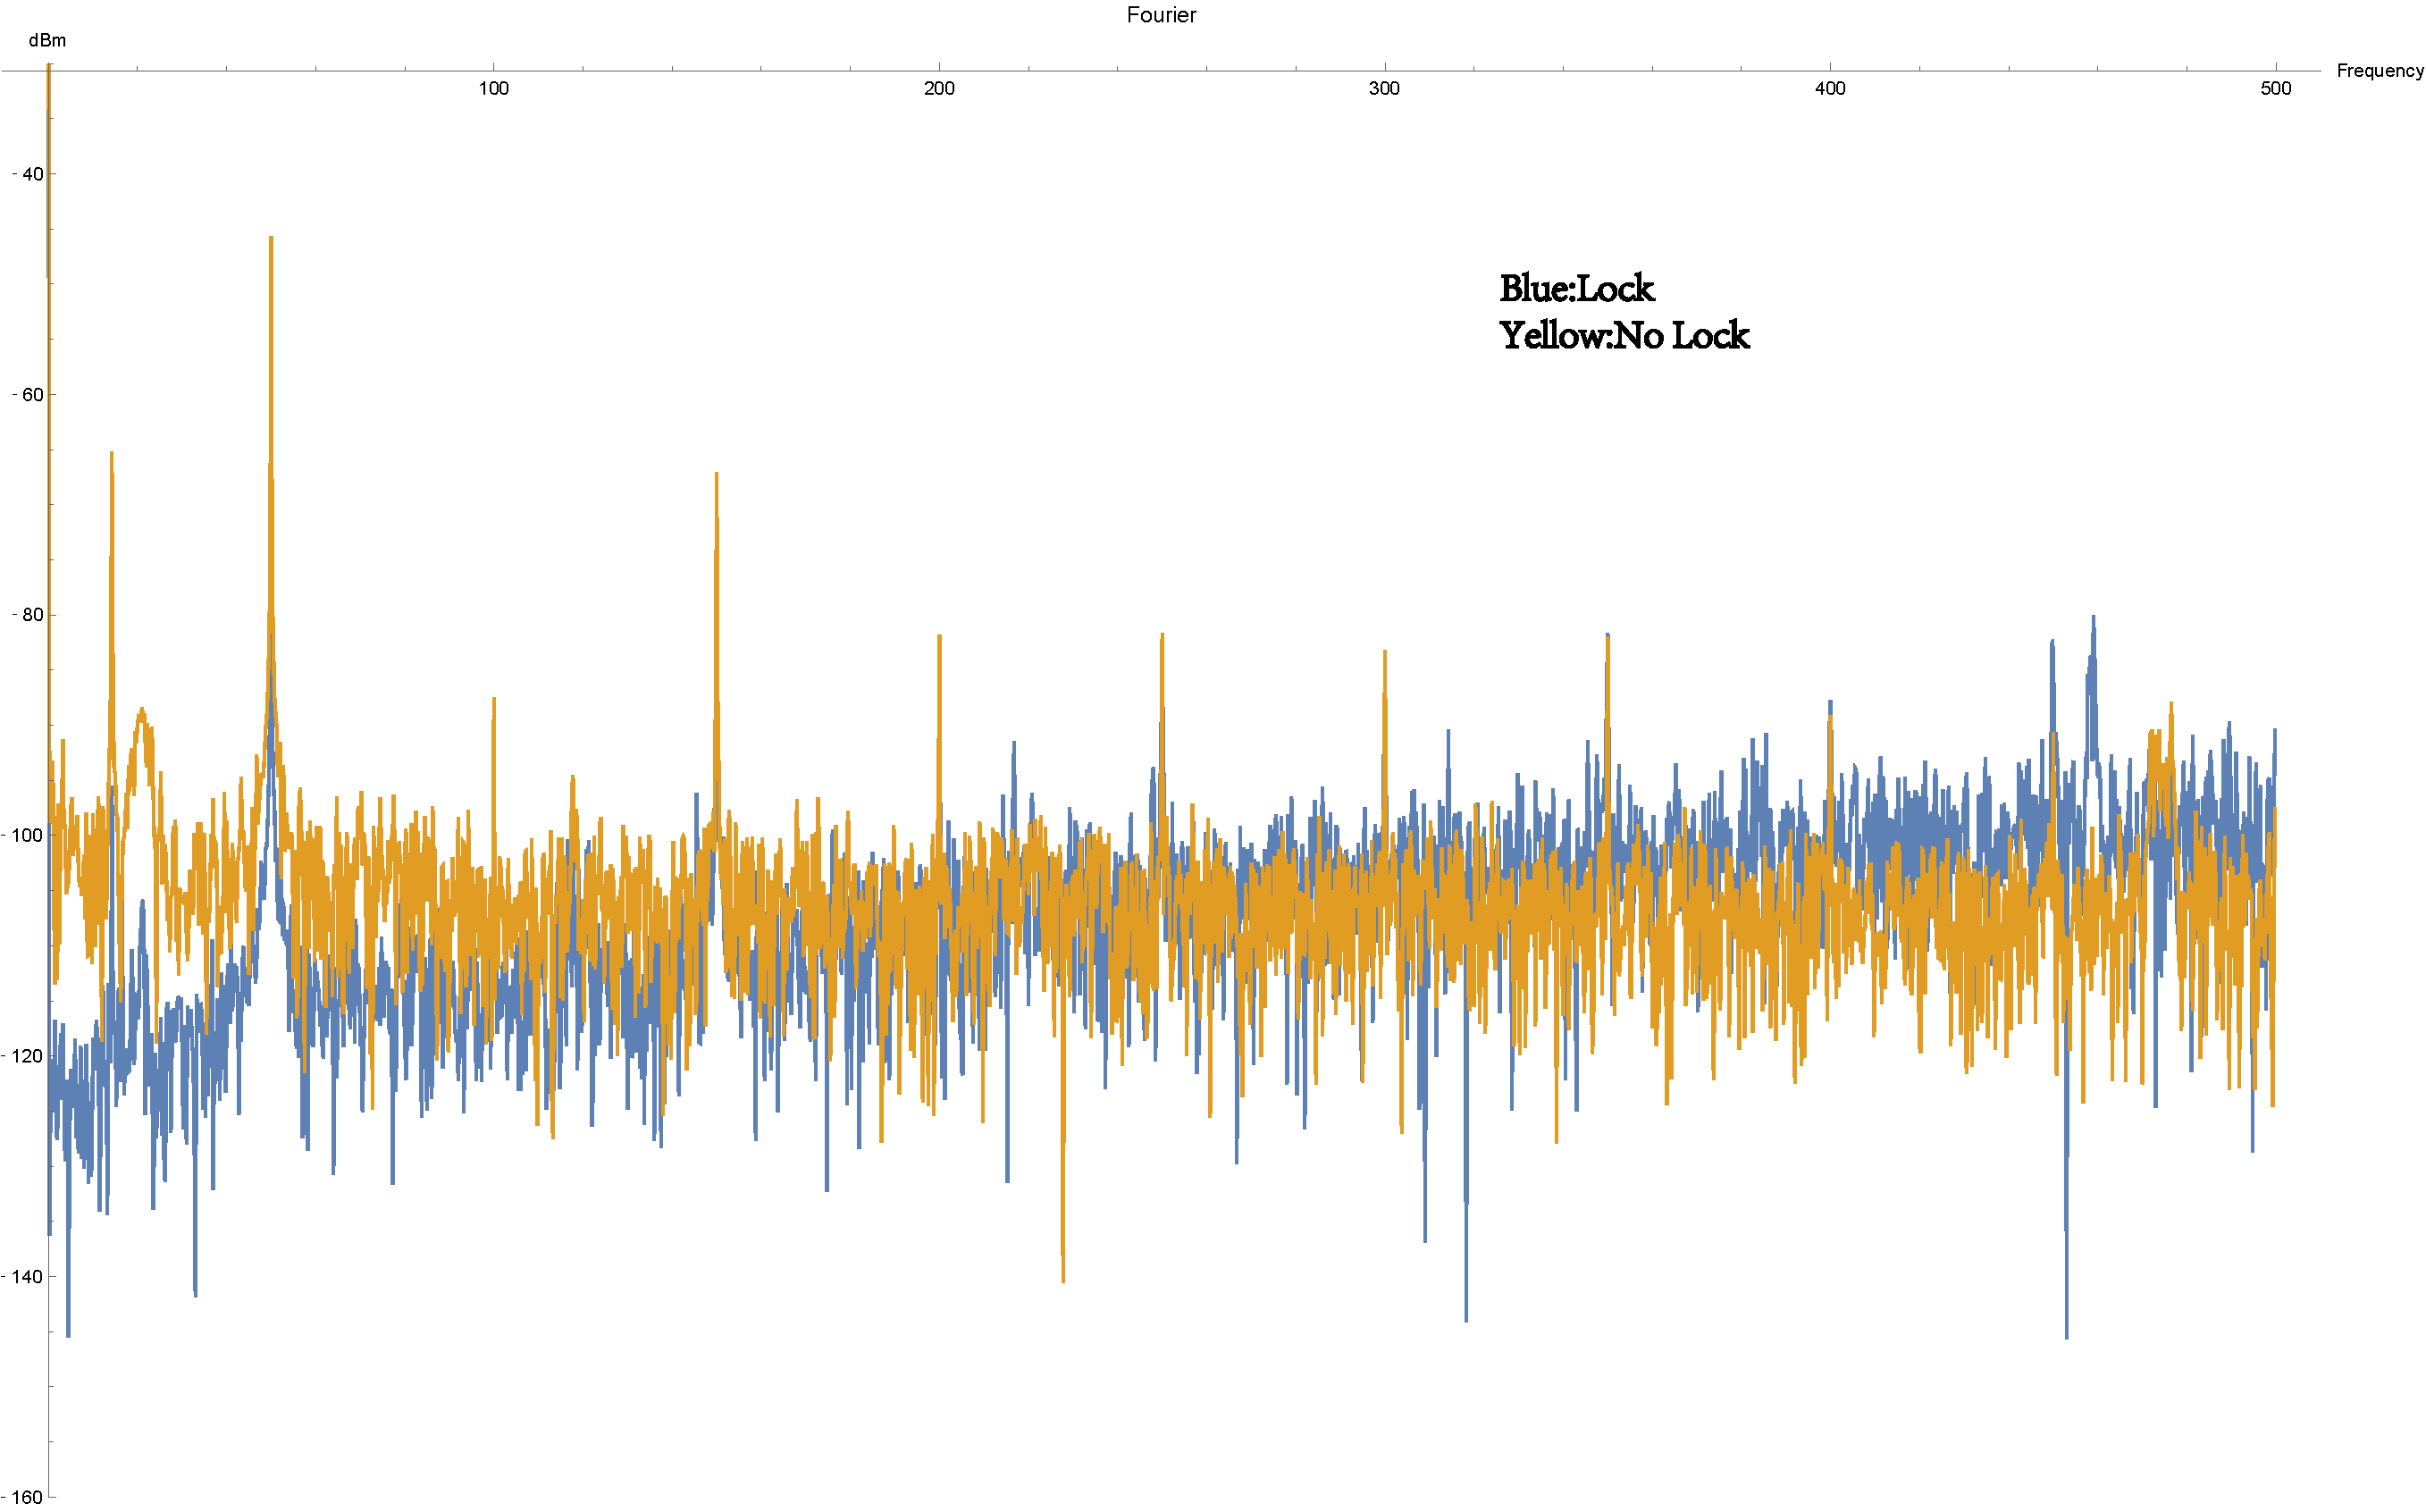
\includegraphics[height=1.75in]{Fourier-Sensor1-Adwin.pdf}
\caption{锁定前后ADWIN通道1磁场数据与频谱对比图}
\label{fig:1204}
\end{figure}
图\ref{fig:1204} RMS噪声:1.5mG->0.42mG


我们发现,整个频率范围内白噪声在锁定后都大于锁定前,在50Hz以下并没有在锁定通道所看见的非常有效的噪声抑制效果,虽然与万用表频谱的形状仍然存在着一定差异,但是这一结论和万用表的结果符合的很好。这说明PID反馈回路确实会对测量的数据产生一定的影响,反馈回路一定程度上过滤了一些低频的数据点,但这些点的缺失对于RMS噪声并没有太大影响。这也说明了锁定后白噪声的确会得到加强,可能的原因是特定频率噪声的能量一部分被抑制掉了,但有部分被均分到白噪声本地,这个均分有可能是通过线圈电流的变化实现的。

在我们的多次测量中,不管是并联还是不并联,锁定后RMS噪声都相差不是很大。在所有的结果中我们也发现,在300Hz以下,锁定对所有比较高的特定频率成分都有抑制作用,对于RMS噪声的抑制,不同设备的测量在相近时间和PID参数下都有较为相似的结果。所以今后对于锁定的效果,我们可以用RMS噪声大小和特定频率噪声大小来评价。

结果也表明有效锁定的范围并不局限于测定点,至少在1cm范围内有效,但是这一测试进行过程中,fluxgate附近没有不锈钢之类的易影响磁场分布的物体,而最后fluxgate工作在science腔上,周围有很多金属物件,这个对于锁定会有一定的影响。

\subsubsection{长期锁定效果}

为了能够得到500Hz范围内噪声功率,我们必须设定万用表的采样周期为1ms,受限于万用表的自身内存大小,总采集时间不能太长,我们一般采集20000个点,代表20s的数据进行分析,只能说明短期的锁定效果较好。环境磁场噪声受到温度变化,气压变化,周围设备是否工作以及附近街道的汽车行驶等的影响,会产生长期漂移,如果磁场锁定能够在这一长期漂移中保证较好的抑制效果,才能说明锁定反馈控制工作稳定性较好,足够robust。图\ref{fig:Multimeter3}是通过数字万用表采集的20000s(约6小时)的数据点,采样周期为1s。

\begin{figure}[htbp]
\centering
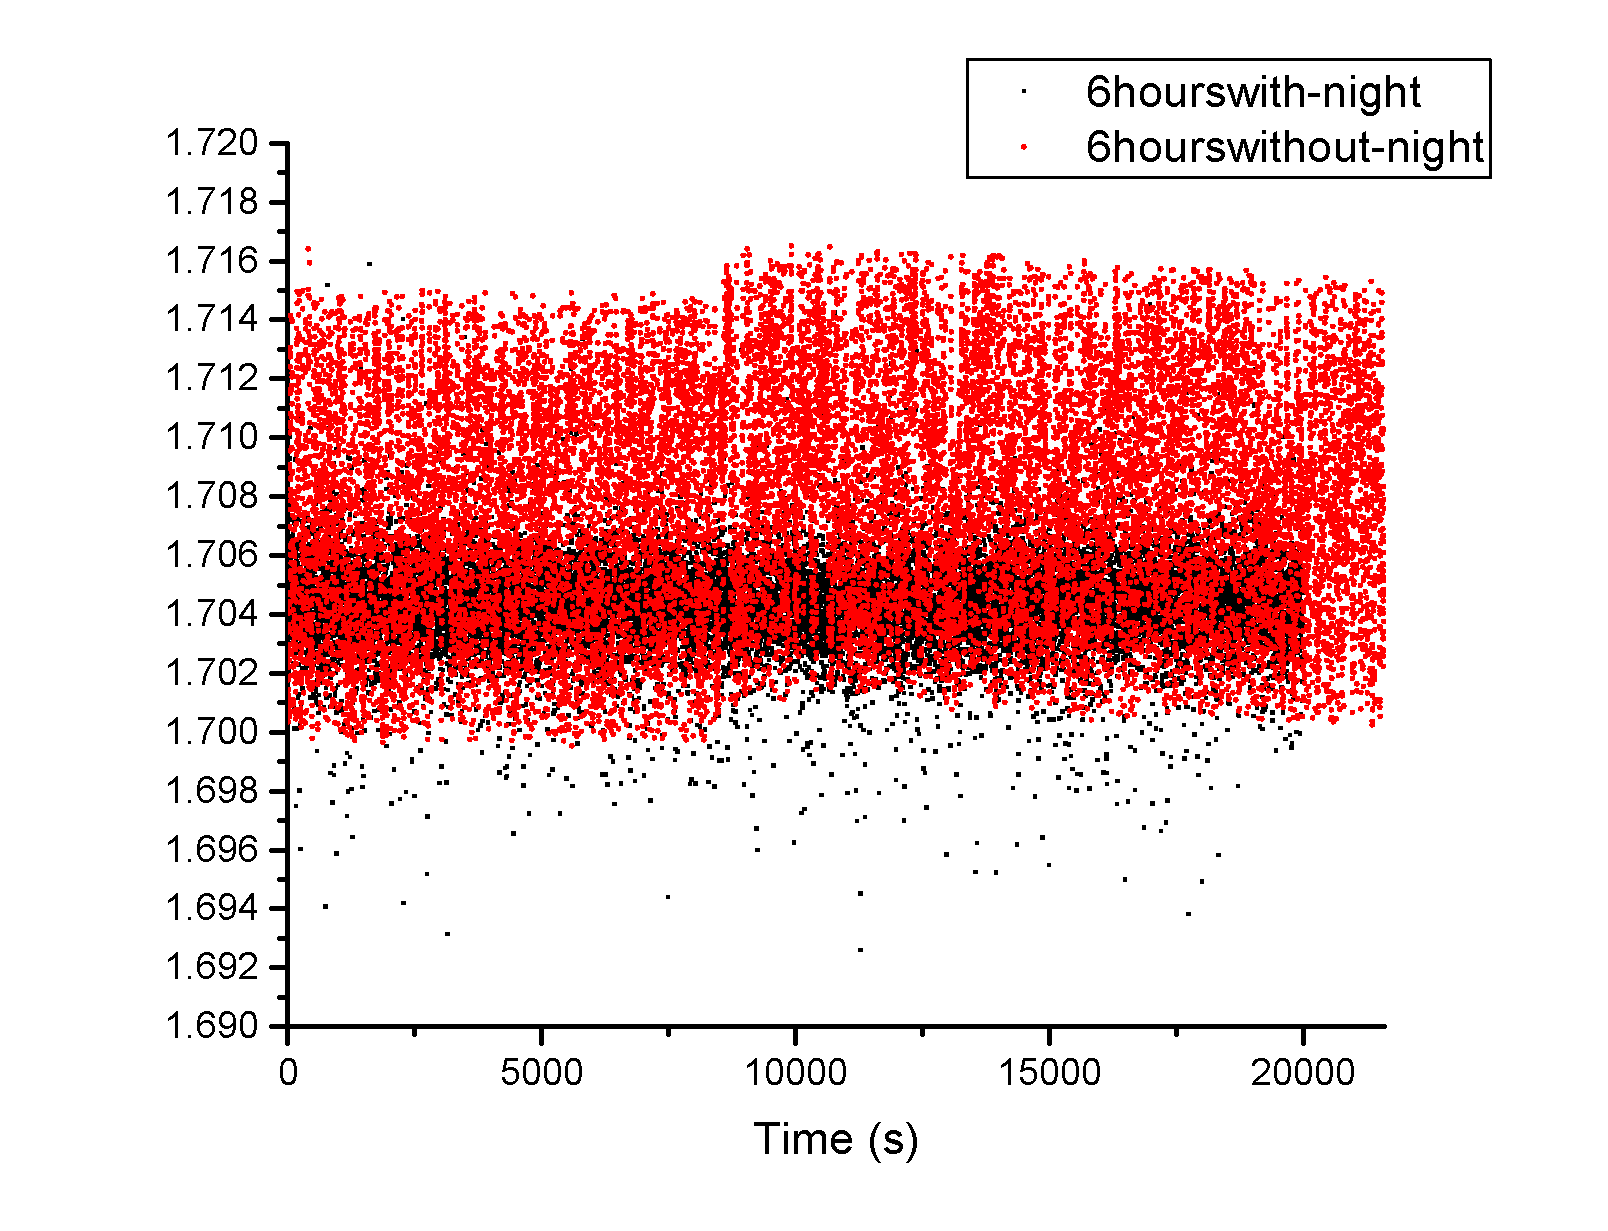
\includegraphics[height=4in]{Longtime}
\caption{长期锁定比较}
\label{fig:Multimeter3}
\end{figure}

图\ref{fig:Multimeter3} RMS噪声:0.78mG->0.3mG

由图可以看出未锁定前长期漂移不大,这可能由于我们测试的时间是周末,大楼内运行设备较少,同时我们实验室地板和墻里有着较好的磁场屏蔽隔层。锁定后可以看出磁场几乎无漂移,RMS噪声依然得到很好的抑制。

\subsubsection{环境磁场噪声时空差异}

以上测试并不是在同一天测量的,在多次测量中我们发现本地的RMS噪声并不是每次都是一样的,以上测试的时候我们都是在实验平台东南角进行,最开始的RMS噪声只有0.78mG左右,但是在后期越变越差,目前高达1.5mG左右,原因未知。

在更早期的时候,我们在真空上方测试过磁场RMS噪声只有0.22mG左右,比东南角要小,但后面没有做进一步测试监控,很难做出准确的分析。

2015.12.03,对平台上部分区域南->北方向的磁场进行测量,结果如下:


\begin{table}[htbp]
\centering

\label{magnetic2}
\begin{tabular}{|c|c|c|}
\hline
位置&S-N磁场大小(G)& RMS Noise(mG)\\
\hline
东南角&0.38  &1.0 \\
\hline
南边靠中间 &0.47  &0.5 \\
\hline
真空第二层 &  -0.49 &1.2 \\
\hline
真空第三层 &  -0.88 &1.3 \\
\hline
\end{tabular}
\caption{不同地点环境磁场噪声大小}
\end{table}

可见不同位置的磁场的大小和噪声水平不一样,同时我们发现在平台上方,磁场的方向发生改变,这是由于附近有一个20L的离子泵,里面的永磁铁对环境磁场的分布产生了影响。

2016.1.15 对平台上Science Chamber位置的磁场进行测量,由于我们实验中将可能会使用竖直方向磁场梯度+微波的方法对单层晶格进行挑选,竖直方向的磁场稳定性会影响微波pump的效率,所以我们这里重点测试了竖直方向上的磁场抖动,测量的磁场平均值为0.444G,方向向下,RMS噪声在0.03$\sim$0.04mG之间。图\ref{fig:1089}是一次测量的数据,磁场断崖式的抖动猜测是因为当时在烘烤science chamber,温控仪的继电器关断电流导致。

\begin{figure}[htbp]
\centering
\includegraphics[height=1.5in]{DATAUP}%
\hspace{0.4in}%   (表示两张图片的中间间距,其中的%不可缺失)
\includegraphics[height=1.75in]{FourierDATAUP}
\caption{20s竖直方向环境磁场变化}
\label{fig:1089}
\end{figure}

从结果上看,频谱上在整个范围内都非常平坦,并且在14Hz左右的峰相对之前南北方向的测量来说也非常小,这从一方面说明了我们实验室南北方向有很强的磁场噪声影响,有可能是旁边机房导致的。

作为对比,我们也测试了该位置南北方向的磁场变化,数据如图\ref{fig:1090}.磁场大小为0.35G,RMS噪声为0.44$\sim$0.46mG左右。

\begin{figure}[htbp]
\centering
\includegraphics[height=1.5in]{SNDATA}%
\hspace{0.4in}%   (表示两张图片的中间间距,其中的%不可缺失)
\includegraphics[height=1.75in]{FourierSNDATA}
\caption{20s南北方向环境磁场变化}
\label{fig:1090}
\end{figure}

从图上可以看到,300Hz以下南北方向的噪声相对较强,这个需要进行一定的补偿锁定。

\subsection{BCS5/10测试结果}

首先,该电流源在出厂时内部是针对2欧的电阻优化内部的PID结构,测试发现,我们的线圈电阻为0.25欧,电感为9$\mu H$,电流源对阶跃信号的响应不是很理想,上升曲线会over damp,上升时间为200us,为此,我们购买了能够承受50w热功率的2欧铝壳电阻来和线圈串联,使得上升时间到达标称的50us,并且消除了振荡。使用34410A测得电流源在2A左右输出时rms噪声为60uA,对全量程来说为12ppm,达到了标称的小于25ppm的指标。

首先我们测量了N175的锁定效果,从adwin测量的结果来看最好时可以将背景噪声从0.94mG抑制到0.2mG左右,对50Hz噪声由有25dB的衰减,如图\ref{fig:1091}.
\begin{figure}[htbp]
\centering
\includegraphics[height=1.5in]{20160420n175data}%
\hspace{0.4in}%   (表示两张图片的中间间距,其中的%不可缺失)
\includegraphics[height=1.75in]{20160420n175}
\caption{N175磁场锁定效果}
\label{fig:1091}
\end{figure}

但是当我们使用BCS进行测量的时候,锁定效果不佳,只能锁定在0.6mG左右,而且锁定后的磁场数据散点图很不均匀。观察发现,这个时候adwin测得不锁定的环境噪声也有很大的问题,峰峰值忽高忽低,测得rms噪声大小也不稳定,而同一时刻由34410A测得的结果一直很稳定,且散点分布均匀。而且这个问题在adwin测量模块AIn-F-8/18上每个通道都有。经过排查,我们发现当我们把adwin模拟输出的某个通道接到N175时,并且这个N175是有±15V供电时,噪声测量才比较稳定,并且和34410A测量结果吻合。

具体原因尚未找到。

解决这个问题之后,我们再次使用BCS5/10进行锁定,当环境噪声为0.8mG时,可以锁定到0.24mG,此时磁场方向为南北方向,如图\ref{fig:1029}.

\begin{figure}[htbp]
\centering
\includegraphics[height=1.5in]{20160428adwinSNdata}%
\hspace{0.4in}%   (表示两张图片的中间间距,其中的%不可缺失)
\includegraphics[height=1.75in]{20160428adwinSN}
\caption{南北方向BCS5/10磁场锁定效果}
\label{fig:1092}
\end{figure}

这个结果还不是很理想,海德堡实验室从0.4mG锁到过0.1mG左右,上海帅实验室锁到过0.05mG,初步怀疑是我们背景噪声过高。为了检验这一点,我们将对东西方向的磁场进行锁定,这个方向上磁场噪声一直都比较小,实验测得为0.4mG左右,目前最好锁定到0.26mG,也就是说本底背景噪声的大小并不影响最好的结果,锁定效果应该是被锁定回路的一些性质所限制。

为此,根据杨兵师兄的建议,我们将采样率从50kHz提高到200kHz,这次观测到磁场噪声最好可以被锁定到0.1mG左右,无论本底噪声是0.26mG还是0.78mG。如图\ref{fig:1093}.

\begin{figure}[htbp]
\centering
\includegraphics[height=1.5in]{20160429adwinEWdata}%
\hspace{0.4in}%   (表示两张图片的中间间距,其中的%不可缺失)
\includegraphics[height=1.75in]{20160429adwinEW}
\caption{200kHz采样下BCS5/10磁场锁定效果}
\label{fig:1093}
\end{figure}

数据点图中可以看见散点都明显的分辨间隔,这是由ADwin数据采集ADC转换的位数所限定的,约为0.3mV,对应0.06mG。
由于CPU运行速度以及内存有限,采样率很难再提的更高。

在测试过程中,我们发现另外一个问题,同一套PID参数下两次时间相近的测试所得到的锁定效果会不一样,我们可以在这次测得rms噪声锁定到了0.11mG,下一次可能就到了0.22mG,再下一次就有0.18mG。这个问题目前原因也不明。

\subsection{下一步计划}

对于PID程序需要进一步优化修改以适应新模块的需要,增加实验中可能需要的功能。另外,对于测量通道测量稳定性问题也需要检查和解决。

\section{总结}

就全部的测试来看,我们可以得到以下结论:
\begin{itemize}
\item 使用BCS5/10我们可以将我们的磁场噪声最好锁定到0.1mG,一般小于0.22mG,对300Hz以下的噪声具有很好的抑制,。
\item 实验室南北方向噪声较强,到1mG左右,除了50Hz以及倍频外,实验室里面在14.2Hz有比较强的磁场噪声。
\item 提高采样率可以有效降低adwin的测量噪声提高锁定效果。
\item Adwin的测量模块只有当输出通道接到通电的N175上测量才会稳定,原因不明。
\item 锁定回路中的测量结果在频谱上会在低频下噪声锁定效果显得比其他设备得出的结果较好。
\item 补偿对于sensor周围1cm的地方效果都会比较好,更远距离没有数据支持,不能做进一步判断。
\end{itemize}





%\section{参考文献}
%%%%%%%%%%%%%%%%%%%%%%%%%%%%%%%%%%%%%%%%%%%%%%%%%%%%%%%%%%%%%%%%
%  参考文献
%%%%%%%%%%%%%%%%%%%%%%%%%%%%%%%%%%%%%%%%%%%%%%%%%%%%%%%%%%%%%%%%


\end{document}

